\begin{figure}[H]
    \centering
    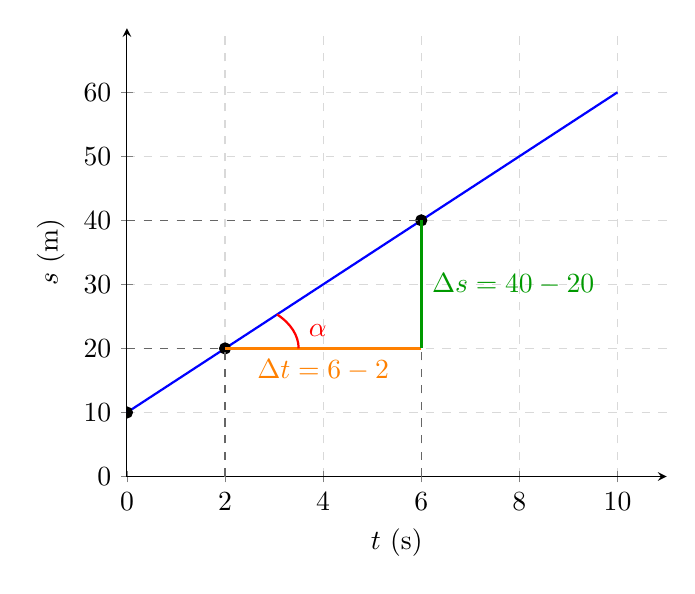
\begin{tikzpicture}
        \begin{axis}[
            axis lines = left,
            xlabel = {$t$ (s)},
            ylabel = {$s$ (m)},
            xmin=0, xmax=11,
            ymin=0, ymax=70,
            xtick={0, 2, 4, 6, 8, 10},
            ytick={0, 10, 20, 30, 40, 50, 60},
            grid = major,
            grid style = {dashed, gray!30}
        ]
            % A Reta do Movimento
            \addplot [domain=0:10, samples=100, color=blue, thick] {10 + 5*x};

            % Ponto Inicial do Intervalo (t=2, s=20)
            \filldraw[black] (axis cs:2,20) circle (2pt);
            \draw [dashed, black!60] (axis cs:2,0) -- (axis cs:2,20);
            \draw [dashed, black!60] (axis cs:0,20) -- (axis cs:2,20);

            % Ponto Final do Intervalo (t=6, s=40)
            \filldraw[black] (axis cs:6,40) circle (2pt);
            \draw [dashed, black!60] (axis cs:6,0) -- (axis cs:6,40);
            \draw [dashed, black!60] (axis cs:0,40) -- (axis cs:6,40);

            % Catetos do Triângulo (Delta t e Delta s)
            % Delta t: horizontal ligando t=2 a t=6 na altura s=20
            \draw [very thick, orange] (axis cs:2,20) -- (axis cs:6,20) 
                node[pos=0.5, below] {$\Delta t = 6 - 2$};
            
            % Delta s: vertical ligando s=20 a s=40 na posição t=6
            \draw [very thick, green!60!black] (axis cs:6,20) -- (axis cs:6,40) 
                node[pos=0.5, right] {$\Delta s = 40 - 20$};

            % Angulo Alfa (ajustado para o novo vértice do triângulo em 2,20)
            \draw [thick, red] (axis cs:3.5, 20) 
                arc [x radius = 1.5, y radius = 7.5, start angle = 0, end angle = 45] 
                node[pos=0.5, right, xshift=2pt] {$\alpha$};

            % Posição Inicial s0
            \filldraw[black] (axis cs:0,10) circle (2pt) node[anchor=east, xshift=-2pt] {$s_0$};
            
        \end{axis}
    \end{tikzpicture}
    \caption{Decomposição do movimento: a velocidade é a razão entre o deslocamento ($\Delta s$) e o intervalo de tempo ($\Delta t$).}
\end{figure}